\documentclass[10pt]{article}
\usepackage[T1]{fontenc}
\usepackage{lmodern,graphicx,microtype,geometry,amsmath,amssymb,amsthm,mathtools,booktabs,array,xcolor,fancyhdr,titlesec,enumitem}
\usepackage[hyphens]{url}
\definecolor{ink}{HTML}{18374A}\definecolor{accent}{HTML}{10655F}
\usepackage[colorlinks=true,urlcolor=accent,linkcolor=accent,citecolor=accent,pdftitle={Beyond Dirichlet GRH: sharp specialization and random symplectic blocks}]{hyperref}
\geometry{letterpaper,inner=.89in,outer=.89in,top=.85in,bottom=.82in}
\newtheorem{theorem}{Theorem}[section]\newtheorem{proposition}[theorem]{Proposition}
\titleformat{\section}{\Large\sffamily\bfseries\color{ink}}{\thesection}{.65em}{}
\titleformat{\subsection}{\large\sffamily\bfseries\color{accent}}{\thesubsection}{.6em}{}
\titleformat{\paragraph}[runin]{\sffamily\bfseries\color{ink}}{}{0pt}{}
\titlespacing*{\section}{0pt}{2.5ex plus .5ex}{1.1ex}
\titlespacing*{\subsection}{0pt}{1.8ex plus .4ex}{.8ex}
\pagestyle{fancy}\fancyhf{}\fancyhead[L]{\small\sffamily\color{ink}Beyond Dirichlet GRH}
\fancyhead[R]{\small\sffamily\color{ink}Torsion, random matrices and Frobenius tests}
\fancyfoot[C]{\small\sffamily\thepage}\setlength{\headheight}{15pt}\renewcommand{\headrulewidth}{.25pt}
\setlength{\emergencystretch}{2.5em}\setlength{\parindent}{1em}
\newcommand{\src}[2]{\href{https://github.com/lsernau/grh-lean/blob/72fead102f663d5c7a407964a13dc0cf9d977207/#1}{#2}}
\newcommand{\prior}[2]{\href{https://github.com/VladimirReshetnikov/ProveIt/blob/274841c1cb137aafbb60ab5f519c51fd42eee98e/docs/incoming/#1}{#2}}
\begin{document}\raggedbottom\thispagestyle{plain}
{\noindent\small\sffamily\bfseries\color{accent}RESEARCH NOTE\hfill 25 NOVEMBER 2026\par}
\vspace{10pt}
{\noindent\fontsize{27}{31}\selectfont\sffamily\bfseries\color{ink}Beyond Dirichlet GRH\par}
\vspace{4pt}
{\noindent\fontsize{15}{19}\selectfont\sffamily\color{ink}Sharp torsion specialization, random symplectic blocks,\\and the reach of one-sided Frobenius tests\par}
\vspace{7pt}{\noindent\color{accent}\rule{\linewidth}{.7pt}\par}\vspace{4pt}
\noindent\textbf{Results.} A valuation estimate used to choose twists in the Lean proof gives two exact answers to questions in the ProveIt reports. For a single integral polynomial the least universally sufficient torsion exponent is $h_0+\lfloor p^{h_0-1}B\rfloor$ at fixed Gauss budget $B$. For simultaneous individual losses over a finite $p$-adic coefficient field, the minimum budget to defeat an entire shell at zero tolerance depends only on the wild part of the ramification index. We compute the price at every rational tolerance by finite congruences. At order four two fields with the same value group and cyclotomic intersection have different prices.

A Fourier estimate used for spanning gives a bound for the joint distribution of rectangular blocks of random finite symplectic matrices. At fixed dimension deficit we compute the exact limiting discrepancy for isotropic blocks. Finally, the sign argument used to locate zeros gives a finite optimization for the part of a nonabelian extension seen by a sparse Frobenius statistic. We identify the precise prime estimate still needed for the splitting field of $X^4-X-1$.

\section{Where the arguments enter the Lean proof}
The public types at revision \texttt{72fead102f66} concern the Riemann zeta function and Dirichlet $L$-functions over $\mathbb Q$. The proof of half-plane nonvanishing compares upper and lower bounds for the same twisted lattice. Short integral forms bound a covolume; a second moment supplies enough forms; and determinants of chains of theta lifts give the lower bound. Comparing them bounds a smoothed sum over prime powers in a progression, weighted by a quadratic twist. Its Mellin transform sees a signed difference of zero multiplicities. Choosing a twist to avoid unwanted zeros makes a one-sided bound sufficient to rule out a proposed zero. The source files and upstream verification record are linked in \cite{repo}. The downstream proofs here are on paper with finite arithmetic checks. We inspected the Lean declarations without rerunning the upstream build.
\begin{center}\small
\begin{tabular}{@{}p{.22\linewidth}p{.36\linewidth}p{.35\linewidth}@{}}\toprule
Source component & Role upstream & Application here\\\midrule
\src{grh/src/New/Congruences/Selmer/RootsOfUnity.lean}{Roots of unity} & Specialize integral polynomials at torsion points within valuation budgets. & Exact order cutoffs and the effect of the coefficient field (Sections 2--3).\\[4pt]
\src{grh/src/New/Spanning/SecondMoment/PositiveType.lean}{Positive type} & Control the frequency of a singular matrix compression in the spanning argument. & Distribution of all entries of a random symplectic block (Section 4).\\[4pt]
\src{grh/src/New/Reduction/Zeros/Criterion.lean}{One-sided zero criterion} & Use signs of real residues in a Mellin transform to exclude zeros. & Optimize which nonabelian factors a restricted prime statistic sees (Section 5).\\\bottomrule
\end{tabular}\end{center}
\paragraph{Two numerical benchmarks.}
At $p=3$ with starting exponent $2$ and budget $1$, the earlier sufficient exponent was $47$. Exponent $5$ is optimal: a degree-$26$ polynomial defeats $2,3,4$, and every allowed polynomial succeeds by $5$. Over $\mathbb F_2$, a square isotropic block of a large random symplectic matrix has a one-dimensional row deficiency with limiting probability $0.419422$; for a uniform binary matrix the probability is $0.577576$. Their difference is the exact limiting total variation distance between the two matrix laws.

\clearpage
\section{The sharp conductor bound for a fixed Gauss valuation}
\label{sec:fixed-radius}

Fix a prime $p$. Normalize the valuation of $\mathbf C_p$ by $v(p)=1$ and
write $v(0)=+\infty$. Set $e_h=(p-1)p^{h-1}$, $r_h=1/e_h$, and
$U_h=\{\zeta:\operatorname{ord}(\zeta)=p^h\}$. For a nonzero polynomial
$g(T)=\sum_n a_nT^n$ with coefficients in $\mathcal O_{\mathbf C_p}$ let
$G_\rho(g)=\min_n(v(a_n)+n\rho)$. The same definition applies to integral
formal series at every $\rho>0$. A shell $h$ is \emph{blocked} at tolerance
$\delta\ge0$ when every $\zeta\in U_h$ satisfies
$v(g(\zeta-1))>G_\rho(g)+\delta$. Equality is a successful specialization.

\paragraph{Theorem (exact worst conductor).}
Fix $h_0\ge1$ and $\rho\ge r_{h_0}$. The smallest value of $G_\rho(g)$
among all integral polynomials blocking the $L$ consecutive shells starting
at $h_0$ at tolerance zero is
\[
                        Lp^{1-h_0}.
\]
Consequently, given $G_\rho(g)\le B$, the least endpoint that guarantees
a successful specialization in $[h_0,H]$ for every $g$ is
\[
                 \boxed{H=h_0+\lfloor p^{h_0-1}B\rfloor.}
\]
Both assertions hold for integral formal series. The same endpoint works
for a series in any finite number of variables, with independent choices
of coordinates on the indicated shells.

The prior \emph{Exact torsion specialization} report gave the sufficient
endpoint $h_0+\lceil p^{h_0}B(h_0+B+2)\rceil$ and left its optimal value
open. The prior \emph{Torsion and zero data} report computed the extremal
loss \emph{within} a shell. Across shells the fixed Gauss valuation
retains the savings from roots on every earlier shell. Keeping these
savings yields an exact balance and the linear answer above.

\subsection{A calculation on one shell}
With a primitive $p^h$th root $\xi$, write $z_a=\xi^a-1$ for unit
residues $a\bmod p^h$. Let $D_h(m)$ be the largest possible value of
\[
   \min_a \sum_{i=1}^m \big(v(z_a-\alpha_i)-r_h\big),
        \qquad v(\alpha_i)=r_h.
\]
The following formula is the shell calculation in the earlier
\emph{Torsion and zero data} report:
\[
 D_h(m)=
 \begin{cases}
  e_h^{-1}\displaystyle\sum_{j=1}^{h-1}e_j\lfloor m/e_j\rfloor,
                    &0\le m<e_h,\\
  +\infty,&m\ge e_h.
 \end{cases}
\]
Here $v(z_a)=r_h$ follows by evaluating $\Phi_{p^h}(1)=p$, since
primitive conjugates yield factors of equal valuation. For each $\alpha_i$,
replace it by a shell point $z_b$ nearest to it. For every $a$,
$v(z_a-z_b)\ge\min(v(z_a-\alpha_i),v(\alpha_i-z_b))
=v(z_a-\alpha_i)$, so the replacement can only raise the minimum.

Now $m$ marks occupy unit residues. Write $N_j(a)$ for the number
congruent to $a$ modulo $p^j$. If $a$ is unmarked, then
$v(z_a-z_b)=p^{v_p(a-b)}/e_h$. Expanding $p^t-1=\sum_{j=1}^t e_j$
shows the excess at $a$ is $e_h^{-1}\sum_{j<h} e_jN_j(a)$.
Follow a least-occupied unit class modulo $p$ and then a least-occupied
child at each subsequent level. This gives
$N_j(a)\le\lfloor m/e_j\rfloor$ simultaneously, and ends at an unmarked
point if $m<e_h$. This proves the upper bound. Conversely, the first $m$
positive integers prime to $p$ give at least $\lfloor m/e_j\rfloor$
marks in every unit class modulo $p^j$, since each successive block of
$e_j$ unit exponents covers every such class. This attains the bound.
For $m\ge e_h$, covering the entire shell gives infinite excess.

\subsection{The exact budget for any finite set of shells}
In fact let $S$ be any nonempty finite set of positive indices with
$\rho\ge\max_{h\in S}r_h$. In increasing order of $h\in S$, define
\[
  m_h=\min\left\{0\le m\le e_h:
  D_h(m)>\delta+\sum_{s\in S,\,s<h}m_s(r_s-r_h)\right\}.
\]
The exact minimum budget for blocking every shell in $S$ is then
\[
                           \sum_{h\in S}m_hr_h.                 \tag{*}
\]
To prove necessity, factor $g=b\prod_i(T-\alpha_i)$ in $\mathbf C_p$.
Gauss multiplicativity gives
$G_u(g)=v(b)+\sum_i\min(u,v(\alpha_i))$. Let $M_h$ count roots of
valuation $r_h$, with multiplicity. Then
$G_\rho(g)\ge G_\rho(g)-G_0(g)\ge\sum_{h\in S}M_hr_h$ by integrality.
At shell $h$ all other roots contribute exactly their Gauss term at $r_h$.
The savings relative to the target include
\[
 G_\rho(g)-G_{r_h}(g)\ \ge\sum_{s\in S,\,s<h} M_s(r_s-r_h).
\]
Thus blocking forces $D_h(M_h)>\delta+\sum_{s<h}M_s(r_s-r_h)$, with
$s$ restricted to $S$. Induction in $S$ gives $M_h\ge m_h$. The
argument permits roots at zero or of negative valuation.

For equality, take on each shell the first $m_h$ unit exponents in the
construction above, and form the monic polynomial with exactly these
shifted roots. Its Gauss valuation is $\sum m_hr_h$. At each selected
shell the savings equal the displayed sum exactly, and the minimum
excess over $G_{r_h}$ is $D_h(m_h)$. The strict inequality in the
recurrence blocks every shell. The coefficients belong to
$\mathbf Q_p(\mu_{p^{\max S}})$.

\subsection{Evaluation for consecutive shells and zero tolerance}
For $h=h_0+k-1$, put $c=p^{1-h_0}$, so $e_k/e_h=c$. We claim
$m_h=e_k$. Assume inductively the previous values have this form.
Their savings at shell $h$ are
\[
   d_h=(k-1)c-\frac{p^{k-1}-1}{e_h}.
\]
Indeed every earlier shell costs $c$ and their total number of marks
is $\sum_{i<k}e_i=p^{k-1}-1$. Direct evaluation gives
\[
  D_h(e_k-1)=
       \frac{(k-1)e_k-(p^{k-1}-1)}{e_h}=d_h.
\]
Here only $j<k$ contribute and $\lfloor(e_k-1)/e_j\rfloor=e_k/e_j-1$
for those $j$. The strict blocking test fails at $e_k-1$. If $k=h$ then
$D_h(e_k)=+\infty$. If $k<h$, the summand with $j=k$ appears, giving
$D_h(e_k)=ke_k/e_h>d_h$. This proves the claim from the first step,
including $p=2$ and $h_0=k=h=1$. Equation~$(*)$ gives $Lc$.
The forced number of roots is also sharp: its sum is
$\sum_{k=1}^L e_k=p^L-1$, achieved by the same monic polynomial.
For polynomials of degree at most $D$ and budget at most $B$, the exact
first guaranteed endpoint is therefore
\[
 h_0+\min\bigl(\lfloor p^{h_0-1}B\rfloor,
                    \lfloor\log_p(D+1)\rfloor\bigr).
\]
A budget $B$ can block precisely up to $\lfloor B/c\rfloor$
initial consecutive shells in the worst case. If this number is zero,
the first shell itself is successful. When $p=3$, $h_0=2$ and $B=1$,
the extremizer blocks levels $2,3,4$ with $2,6,18$ roots respectively.
Level $5$ is guaranteed, improving the previous sufficient level $47$.

\paragraph{Passing to power series and several variables.}
For a fixed finite set of shells and a nonzero integral series, truncate
after degree $N$ with $(N+1)\min_{h\in S} r_h>G_\rho(g)+\delta$.
The tail has larger valuation than the comparison threshold at every
test point, and the truncation preserves $G_\rho$. This transfers the
polynomial result to series, including the sharpness examples.

In several variables, choose a coefficient $a_{\mathbf n}$ attaining the
weighted Gauss minimum $A=\min_{\mathbf n}(v(a_{\mathbf n})+\rho|\mathbf
n|)$. It exists since the coefficients are integral and $\rho>0$.
Within the first variable take the series $b(T_1)$ obtained by fixing all
other indices at $(n_2,\ldots,n_d)$. Then $G_\rho(b)+
\rho\sum_{j>1}n_j=A$. The one-variable theorem selects $z_1$ with
$v(b(z_1))\le G_\rho(b)$, so the remaining Gauss minimum is at most
$A$. Successive evaluation and induction give the same endpoint
independently in every coordinate. A polynomial depending on one
coordinate already forces the stated worst endpoint. Applying this to
a finite product gives an aggregate valuation bound by Gauss
multiplicativity.

\paragraph{Relation to earlier maximum principles.}
Kriz and Nordentoft, \emph{Horizontal $p$-adic $L$-functions},
arXiv:2310.20678v3, Propositions 2.7 and 2.11, establish discrete maximum
principles for Fourier transforms of measures on finite abelian groups.
In the cyclic case their second proposition gives the one-shell threshold
$p^{1-h}$ relative to the trivial-character value. Here the reference
is the coefficient Gauss valuation at positive radius, and the proof
computes the obstruction from every previous shell and realizes the
sharp cost simultaneously. The optimality claim concerns the explicit
extremal problem above.   

\section{The exact price over a finite coefficient field}
\label{sec:field}
Let $K/\mathbb Q_p$ be finite, with integer ring $\mathcal O_K$, absolute ramification index $e$ and finite residue field $k$. Continue to normalize $v(p)=1$. Put $N_h=\varphi(p^h)$ and $r_h=1/N_h$. A finite packet consists of nonzero $g_i\in\mathcal O_K[T]$ and witnesses $x_i$ in $\mathbf C_p$ with $v(x_i)\ge\rho>0$ and $t_i=v(g_i(x_i))<\infty$. Its budget is $\sum_i t_i$. At a point $z=\zeta-1$, measure the loss by
\[
                   \sum_i \max(0,v(g_i(z))-t_i).
\]
A packet blocks a shell if this loss exceeds $\epsilon$ at \emph{every} primitive point on it. Write $C_K(S,\epsilon)$ for the minimum budget to block a nonempty finite set $S$ of shells, all with $r_h\le\rho$. Each polynomial has its own witness. This is the simultaneous selection problem in the earlier reports \cite{packet,fieldprior}. The use of the positive part is essential because a saving on one polynomial cannot offset a loss on another.

\begin{theorem}\label{th:ram}
For every finite $K/\mathbb Q_p$ and every eligible $S$,
\[
 \boxed{\quad C_K(S,0)=\sum_{h\in S}p^{-\min(v_p(e),\,h-1)}.\quad}
\]
All the extremizing witnesses may be taken to be zero. In particular, on shells $h\ge1+v_p(e)$ a unit of obstruction costs exactly $p^{-v_p(e)}$ per shell. For an interval starting at such an $h_0$, the least endpoint guaranteeing some specialization with zero positive excess for every packet of budget at most $B$ is $h_0+\lfloor p^{v_p(e)}B\rfloor$.
\end{theorem}

\paragraph{How a shell is charged.}
For $g=b\prod_\alpha(T-\alpha)$, write $G_u(g)=v(b)+\sum_\alpha\min(u,v(\alpha))$. This follows from multiplicativity of the Gauss valuation. At a point $z$ of valuation $r$, the number $v(g(z))-G_r(g)$ is a sum of nonnegative terms; only roots of valuation $r$ can contribute. Since $t_i\ge G_\rho(g_i)\ge G_r(g_i)$, this sum dominates each individual positive loss. Collect the matching roots for the whole packet, including multiplicities. Their monic product $P_h\in\mathcal O_K[T]$ is defined over $K$ because the multiset is Galois-stable. Put $m_h=\deg P_h$. Then
\begin{align}
 &\sum_i\max(0,v(g_i(z))-t_i)\ \le\ v(P_h(z))-m_h r_h, \label{eq:reduce}\\
 &\sum_{h\in S}m_h r_h
 \ \le\ \sum_i\bigl(G_\rho(g_i)-G_0(g_i)\bigr)\ \le\ \sum_i t_i. \label{eq:cost}
\end{align}
A root at valuation $r_h$ contributes exactly $r_h$ to the first difference in \eqref{eq:cost}; all other contributions are nonnegative, including those of roots of negative valuation. Conversely, monic polynomials with all roots on their designated radius have $v(P_h(0))=m_hr_h$. Using one per shell and taking witnesses at zero attains the sum of the individual costs whenever each designated shell is blocked. This proves additivity for any tolerance.

\paragraph{Why only the wild part of $e$ survives.}
Fix $h$ and abbreviate $N=N_h$, $r=1/N$, $g=\gcd(N,e)$ and $d=N/g$. Set $\pi=\xi-1$ for a primitive $p^h$th root $\xi$. If $P(T)=\sum_{j=0}^m c_jT^j$ is monic with all its roots of valuation $r$, then $\pi^{-m}P(\pi X)$ is integral with monic reduction over the algebraic closure of the residue field. Its constant term is a unit. A coefficient can survive reduction only if $v(c_j)=(m-j)/N$. Since $v(K^\times)=e^{-1}\mathbb Z$, this forces $d\mid m-j$. The constant term gives $d\mid m$. The reduction is therefore $Q(X^d)$, where $Q$ is monic of degree $m/d$.

For each exponent $a$ prime to $p$, the geometric series gives
$\overline{(\xi^a-1)/\pi}=\bar a$. If $P$ blocks the shell relative to $mr$, the reduction must vanish on $\mathbb F_p^\times$. The $d$th powers of this group have size $(p-1)/\gcd(p-1,d)=\gcd(p-1,e)$. Thus $m/d\ge\gcd(p-1,e)$. Writing $s=\min(v_p(e),h-1)$, this says $m/N\ge p^{-s}$. Equations \eqref{eq:reduce} and \eqref{eq:cost} apply the bound to every packet.

For the matching binomial choose $m=N/p^s$. The shifted cyclotomic polynomial $\Phi_{p^h}(1+T)$ is Eisenstein with constant coefficient $p$, so $\overline{\pi^N/p}=-1$. This holds at every primitive point. There is $c\in K$ with $v(c)=p^{-s}$ and $\overline{c^{p^s}/p}=-1$. Indeed, start with a uniformizer to the power $e/p^s$ and adjust by a unit; the $p^s$th-power map is bijective on $k$. For every $z=\xi^a-1$ the unit $z^m/c$ reduces to $1$, since its $p^s$th power does. All roots of $T^m-c$ have valuation $r$, and
\[
                   v(z^m-c)>p^{-s}=v(c).
\]
This polynomial and the witness zero attain the lower bound. The strict inequality also explains why equality of the total budget with the obstruction cost allows failure of selection. \hfill$\square$

\subsection{An exact finite calculation at every tolerance}
\label{sec:algorithm}
For positive rational $\epsilon$, the following gives a finite computation of $C_K(S,\epsilon)$ over an explicitly presented local field. It also works at $\epsilon=0$. It avoids enumeration of packet sizes, degrees of arbitrary input polynomials, or possible witnesses.

\begin{proposition}\label{prop:mod}
For shell $h$ set $L=K(\xi)$, $E=e(L/\mathbb Q_p)$, and choose a uniformizer $\varpi$ of $L$. For each $m=1,\ldots,N_h$ form
\[
 t=\big\lfloor E(mr_h+\epsilon)\big\rfloor+1,\qquad
 R=\operatorname{image}(\mathcal O_K\longrightarrow\mathcal O_L/(\varpi^t)).
\]
Let $V_j=((\xi^a-1)^j)_a$ in $(\mathcal O_L/(\varpi^t))^{N_h}$, with $a$ ranging over the units modulo $p^h$. Take the first $m=m_h^*$ satisfying
\[
                 -V_m\ \in\ R V_0+\cdots+R V_{m-1}.
\]
Then $C_K(S,\epsilon)=\sum_{h\in S}m_h^*/N_h$.
\end{proposition}
\begin{proof}
Membership asserts precisely the existence of a monic integral polynomial $P$ of degree $m$ with $v(P(z))>mr_h+\epsilon$ at every test point. The full cyclotomic polynomial shifted by one succeeds at $m=N_h$. If some root of $P$ has a valuation different from $r_h$, its contribution $v(z-\alpha)-r_h$ is either zero or negative at every test point. Removing all such roots leaves a monic integral polynomial over $K$ which still passes its own strict test. Hence a first successful polynomial has all roots on the radius. The reduction \eqref{eq:reduce} implies that every blocking packet has at least $m_h^*$ matching roots at this radius (trivially so if its count exceeds $N_h$). The budget inequality gives necessity, and the successful polynomials used separately with witness zero give attainment.
\end{proof}
Only finite rings and linear membership occur here. The coefficient ring is $\mathcal O_K/\mathfrak p_K^{\,\lceil t/e(L/K)\rceil}$. Enumeration of its $m$-tuples is sufficient; linear algebra over a discrete valuation ring is often cheaper. Checking a single representative per $\operatorname{Gal}(L/K)$-orbit gives the same answer. The complexity can grow rapidly with $h$. Section~\ref{sec:dyadic} evaluates the test in closed form for a shell where the arithmetic of $K$ already matters.

\paragraph{One fixed polynomial over the specified field.}
Proposition~\ref{prop:mod} also makes the recurrence in Section~2 exact over $K$. Let $d_h(t)$ be the first successful degree in the congruence test at tolerance $t$. For $h\in S$ in increasing order set
\[
 n_h=d_h\!\left(\epsilon+\sum_{\substack{j\in S\\j<h}}
                         n_j(r_j-r_h)\right).
\]
The least $G_\rho$ of a \emph{single} polynomial over $\mathcal O_K$ blocking all $S$ relative to the common fixed value $G_\rho+\epsilon$ is $\sum_h n_hr_h$. To see necessity, extract the same-radius monic factor at each shell. The savings already accumulated on earlier shells are at least the sum in the recurrence, by induction and $r_j>r_h$. The extracted factor must therefore pass the local test at that effective tolerance, so it has degree at least $n_h$. Conversely take the product of the local extremizers found by the tests. Their roots all have the designated radii, giving exactly those savings and the claimed fixed Gauss valuation. The finite computation thus covers both conventions for adding the losses.

\subsection{Primitive fourth roots and the quadratic defect of \texorpdfstring{$-1$}{-1}}
\label{sec:dyadic}
Take $p=2$, $h=2$, $r=1/2$, and any finite extension $K/\mathbb Q_2$. Define the truncated quadratic defect
\[
             d_K=\max_{a\in\mathcal O_K}\min\{2,v(a^2+1)\},
             \qquad \eta_K=(d_K-1)/2 .
\]
The maximum exists since only finitely many residues modulo $4\mathcal O_K$ matter; $a=1$ gives $d_K\ge1$.

\begin{theorem}\label{th:fourth}
For all $\epsilon\ge0$ the minimum blocking budget on this shell equals
\[
 C_K(\{2\},\epsilon)=
 \begin{cases}
   1/2,&0\le\epsilon<\eta_K,\\
   1,&\epsilon\ge\eta_K.
 \end{cases}
\]
\end{theorem}
\begin{proof}
The two points are $i-1$ and $-i-1$. Write a potential linear center as $a-1$. The distances have valuations $v(a-i)$ and $v(a+i)$. Their sum is $v(a^2+1)$ and their minimum is at most $1$, as the two targets differ by $2i$. If the minimum is less than $1$ the two valuations are equal. Thus their minimum is exactly $\tfrac12\min(2,v(a^2+1))$, including $a=\pm i$. A monic linear polynomial succeeds in Proposition~\ref{prop:mod} precisely for $\epsilon<\eta_K$. A monic quadratic with both targets as roots always succeeds. These are all possible first successful degrees.
\end{proof}

\begin{center}
\begin{tabular}{@{}lccc@{}}\toprule
$K=\mathbb Q_2(\sqrt D)$, by radicand & $d_K$ & $\eta_K$ & $C_K(\{2\},1/4)$\\\midrule
$D=5$ & $1$ & $0$ & $1$\\
$D=2,-2,10,-10$ & $3/2$ & $1/4$ & $1$\\
$D=-1,3$ & $2$ & $1/2$ & $1/2$\\\bottomrule
\end{tabular}
\end{center}
\noindent These are representatives of all seven quadratic extensions of $\mathbb Q_2$ (the square class of $3$ is that of $-5$). The table can be verified in sixteen residues per field. For even $D$ the basis is $1,\sqrt D$; for $D=-1,3$ use $1,\sqrt D-1$. In both cases the second basis element $\lambda$ is an Eisenstein uniformizer, giving $v(b+c\lambda)=\min(v_2(b),v_2(c)+1/2)$. For $D=5$ use $\lambda=(1+\sqrt5)/2$. Its irreducible reduction gives the minimum of the two coefficient valuations. Thus computing $a^2+1$ with both basis coefficients of $a$ in $\{0,1,2,3\}$ proves the table by finite arithmetic.

\paragraph{Why the cyclotomic intersection loses information.}
The two fields $K_1=\mathbb Q_2(\sqrt3)$ and $K_2=\mathbb Q_2(\sqrt{10})$ have the same residue field and value group. Both meet $\mathbb Q_2(\mu_{2^\infty})$ only in $\mathbb Q_2$. Indeed the three quadratic subfields of the tower correspond to $-1,2,-2$: for $n\ge3$ the group $(\mathbb Z/2^n)^\times$ has exactly three index-two subgroups and all three fields already lie at level $8$. Their square classes differ from those of $3$ and $10$. Nevertheless the strict tolerance $1/4$ separates the two fields. In $K_1$ the center $\sqrt3-1$ has distance valuation $1$ from both targets. In $K_2$ the center $\sqrt{10}$ has distance valuation $3/4$ from both since
\[
 v\big((1+\sqrt{10})^2+1\big)=v(12+2\sqrt{10})=3/2 .
\]
No element of $K_2$ can improve this: its difference from $\sqrt{10}$ has valuation in $\tfrac12\mathbb Z$ or is zero. The ultrametric inequality with unequal valuations then bounds its proximity to each target by $3/4$. The pair answers the question in \cite{packet} about whether the cyclotomic intersection and allowed coefficient valuations determine the cost at positive tolerance.


\section{Which blocks of a random symplectic matrix look uniform?}

In a symplectic space a change of basis preserves alternating pairings. How many matrix entries can be observed together before those constraints become detectable? Over a fixed finite field we obtain a uniform range for all rectangular compressions. For isotropic blocks at a fixed distance from the boundary we determine the exact limiting total variation distance. The event that the matrix loses precisely one row of rank accounts for that entire distance in the limit. The input from the repository is the Fourier argument in \path{New/Spanning/SecondMoment/PositiveType.lean}, lines 102--136. There it bounds one additive character sum and is then used to estimate the mass of singular square compressions. Passing to ordered frames makes it possible to control the law of the entire matrix.

Let $V=\mathbb F_q^n$, let $G$ act on $V$ by $\pi$, and fix injections $A:\mathbb F_q^a\to V$ and $B:\mathbb F_q^b\to V^*$. For $g\in G$ let $M(g)$ be the $b\times a$ matrix whose $(i,j)$ entry is $(Be_i)(\pi(g)Ae_j)$. Take a probability mass function $\mu$ on the finite group $G$ of positive type, meaning that $(\mu(g^{-1}h))_{g,h\in G}$ is a positive semidefinite matrix. Uniform measure is one example. For $1\le j\le \min(a,b)$ write $\alpha_j$ for the maximum $\mu$-mass of the pointwise stabilizer of an independent ordered $j$-tuple in $\operatorname{im}A$, and $\beta_j$ for the analogous quantity in $\operatorname{im}B$ under the dual action. Write $R_j(a,b)$ for the number of $b\times a$ matrices of rank $j$.

\medskip\noindent\textbf{Distribution bound.}
If $g$ has law $\mu$ and $U$ is uniform on all $b\times a$ matrices, then
\[
 d_{\rm TV}(M(g),U)\le
 \frac12\left(\sum_{j=1}^{\min(a,b)} R_j(a,b)\, q^{nj}\alpha_j\beta_j\right)^{1/2}.
\]

\emph{Proof.}
A rank-$j$ matrix defining a nontrivial Fourier character factors as a sum of $j$ rank-one matrices with independent left and independent right vectors. For a fixed nontrivial additive character $\psi$ of $\mathbb F_q$, its value on $M(g)$ becomes $\psi(y(\pi(g)z))$ on $W=V^j$, for the corresponding frame $z$ and covector frame $y$ with the diagonal actions. Put $D=|W|$. In $\ell^2(W)$ take the unit Fourier vectors $c_v(w)=D^{-1/2}\psi(-v(w))$ and the point masses $e_w$. Choose vectors $u_g$ with Gram matrix $\mu(g^{-1}h)$, with inner product conjugate-linear in the first argument. The inner product of
\[
 \sum_{g\in G} c_{g y}\otimes u_g
       \quad\hbox{and}\quad
 \sum_{h\in G} e_{h z}\otimes u_h
\]
is $|G|D^{-1/2}\sum_t\mu(t)\psi(y(\pi(t)z))$.
Their squared norms are $|G|\mu(\operatorname{Stab}y)$ and $|G|\mu(\operatorname{Stab}z)$ by orthonormality. Cauchy--Schwarz therefore bounds the squared modulus of the Fourier coefficient by $D\alpha_j\beta_j$. The $\ell^1$--$\ell^2$ inequality and Parseval give the displayed estimate, since the uniform distribution has zero Fourier coefficient at every nontrivial character.\hfill$\square$

\medskip\noindent\textbf{Symplectic compression theorem.}
For even $n$, $g$ uniform in $\operatorname{Sp}_n(\mathbb F_q)$, and arbitrary $A,B$ as above with $a+b\le n$, an absolute constant $C$ gives
\[
 d_{\rm TV}(M(g),U)\le C q^{-(n+1-a-b)/2}.
\]
Thus $n-a-b\to\infty$ suffices at fixed $q$, uniformly in both subspaces. For every fixed integer $c\ge0$, the dimensions $n=2m$, $a=m$, $b=m-c$ admit isotropic choices such that the distance stays bounded away from zero as $m\to\infty$.

\emph{Proof of the upper bound.}
The symplectic form identifies the dual action with the given one. By Witt extension, the orbit of an independent $j$-frame consists of all independent frames with its prescribed alternating Gram matrix. Once $i-1$ independent vectors have been specified, the pairings with the next vector give $i-1$ independent linear constraints. Of the $q^{n-i+1}$ solutions at most $q^{i-1}$ are in the previous span. Since $j\le n/2$, every orbit has size at least
\[
 q^{nj-j(j-1)/2}\prod_{i=1}^j(1-q^{2i-2-n})
 \ \ge\ q^{nj-j(j-1)/2}\prod_{k\ge1}(1-2^{-2k}).
\]
Each stabilizer mass is the reciprocal of its orbit size. Factoring rank-$j$ matrices through $\mathbb F_q^j$ and dividing by $|\operatorname{GL}_j(\mathbb F_q)|$ gives
$R_j(a,b)\le q^{j(a+b-j)}/\prod_{k\ge1}(1-2^{-k})$.
Substitution leaves a geometric sum $\sum_{j\ge1}q^{-j(n+1-a-b)}$, as claimed.\hfill$\square$

\emph{Proof of the obstruction.}
Under the symplectic identification take $\operatorname{im}A$ Lagrangian and $\operatorname{im}B=W_0$ isotropic of dimension $m-c$. Then $L=g\operatorname{im}A$ is a uniform Lagrangian. Full row rank of $M(g)$ means $L\cap W_0=0$, since $L^\perp=L$. The number of Lagrangians in dimension $2m$ is $\prod_{k=1}^m(q^k+1)$, as follows by counting pairs of a Lagrangian and a line in it and passing to the line's symplectic quotient. A fixed $i$-dimensional subspace of $W_0$ lies in $L$ with probability $1/\prod_{k=m-i+1}^{m}(q^k+1)$, by the same quotient argument. Subspace-lattice M\"obius inversion gives the full-rank probability
\[
 P_{m,c}=\sum_{i=0}^{m-c}
  \frac{(-1)^i q^{i(i-1)/2}\genfrac{[}{]}{0pt}{}{m-c}{i}_{q}}
       {\prod_{k=m-i+1}^{m}(1+q^k)},
\]
where the Gaussian coefficient counts $i$-subspaces of $W_0$ and the M\"obius function in dimension $i$ is $(-1)^i q^{i(i-1)/2}$. For $c=0$ the probability also has the elementary form $\prod_{k=1}^m(1+q^{-k})^{-1}$, since there are $q^{m(m+1)/2}$ Lagrangian complements, parametrized by symmetric matrices.

Set $Q=q^{-1}$. The $i$th term converges to $(-Q^{c+1})^i/\prod_{k=1}^i(1-Q^k)$ and is bounded in absolute value by $Q^{(c+1)i}/\prod_{k\ge1}(1-Q^k)$. These facts follow by extracting the highest powers of $q$ in the Gaussian coefficient and the denominator. Dominated convergence and the power-series identity
$\sum_{i\ge0}z^i/\prod_{k=1}^i(1-Q^k)=\prod_{k\ge0}(1-zQ^k)^{-1}$
for $|z|<1$ yield
\[
 \lim_{m\to\infty}P_{m,c}=\prod_{k=c+1}^\infty(1+q^{-k})^{-1}.
\]
For the uniform rectangular matrix the full-rank probability is $\prod_{k=c+1}^{m}(1-q^{-k})$. The two positive limits have ratio $\prod_{k=c+1}^\infty(1-q^{-2k})^{-1}>1$. Their difference is a lower bound for limiting inferior total variation.\hfill$\square$

\medskip\noindent\textbf{Exact limiting distance for the isotropic family.}
Continue with $a=m$, $b=m-c$, $n=2m$ and fixed $q,c$. Then the limiting total variation distance of the full matrix equals
\[
 \frac{Q^{c+1}}{1-Q}
 \left(\prod_{j=c+2}^{\infty}(1-Q^j)
       -\frac{1}{\prod_{j=c+1}^{\infty}(1+Q^j)}\right),
 \qquad Q=q^{-1}.
\]
At fixed $q$, this is asymptotic to $Q^{2c+2}/(1-Q)$ as $c\to\infty$, with the limit in $m$ taken first.

\emph{Proof.}
Witt extension realizes every change of coordinates in each of the two isotropic subspaces by a symplectic automorphism. Left and right invariance of uniform $g$ therefore make its compression uniform conditional on its rank, since left and right general linear transformations act transitively on each rank. The uniform rectangular model has the same conditional laws. Hence total variation of the full matrices equals total variation of their row deficiencies $d=b-\operatorname{rank}M$.

Let $s_m(d)$ and $u_m(d)$ be the two deficiency probabilities. Each possible intersection $D=L\cap W_0$ of dimension $d$ gives a symplectic quotient $D^\perp/D$ of dimension $2(m-d)$, with the image of $W_0$ isotropic of dimension $m-d-c$. Conditional on $D\subseteq L$, the Lagrangian $L/D$ is uniform there. In the rectangular model, specifying a $d$-dimensional left kernel first requires the random map $\mathbb F_q^b\to\mathbb F_q^m$ to vanish on it, then to be injective on its quotient. Therefore, for $0\le d\le m-c$,
\[
 s_m(d)=\genfrac{[}{]}{0pt}{}{m-c}{d}_{q}\frac{P_{m-d,c}}{\prod_{j=m-d+1}^{m}(1+q^j)},\qquad
 u_m(d)=\genfrac{[}{]}{0pt}{}{m-c}{d}_{q} q^{-md}\prod_{j=c+d+1}^{m}(1-Q^j).
\]
Both families are tight on the nonnegative integers. The expected number of lines in the left kernel is \( \genfrac{[}{]}{0pt}{}{m-c}{1}_{q}/(q^m+1)\) in the symplectic model, by the one-line quotient count, and \( \genfrac{[}{]}{0pt}{}{m-c}{1}_{q} q^{-m}\) for a uniform matrix. Both remain bounded as $m\to\infty$, while a $d$-dimensional kernel contains $(q^d-1)/(q-1)$ lines. Pointwise convergence of both mass functions, which follows from the displayed formulas, thus implies convergence in total variation to their respective limiting laws.

Write $s(d),u(d)$ for the limits and $R_d=s(d)/u(d)$, with $u(d)>0$. Taking ratios gives
\[
 R_0=\prod_{j=c+1}^{\infty}(1-Q^{2j})^{-1}>1,\qquad
 \frac{R_{d+1}}{R_d}=Q^{-d}(1-Q^{c+d+1}).
\]
Set $t=Q^{c+1}$. Retaining the first two factors of $R_0$ yields $R_2\ge[Q(1+t)(1+Qt)]^{-1}>1$, since $Q\le1/2$ and $t\le Q$. For $d\ge1$ the successive ratio is at least $Q^{-1}(1-Q^2)>1$. All deficiencies except possibly $d=1$ therefore have excess mass in the symplectic law, with strict excess at $d=0$. As both limiting laws have total mass one, the distance is exactly $u(1)-s(1)$. Substitution gives the stated expression. Finally,
$\prod_{j=c+2}^\infty(1-Q^j)=1-Qt/(1-Q)+O_q(t^2)$ and
$\prod_{j=c+1}^\infty(1+Q^j)^{-1}=1-t/(1-Q)+O_q(t^2)$
by the convergent logarithmic expansions. Their difference is $t+O_q(t^2)$, proving the asymptotic.\hfill$\square$

\begin{figure}[htbp]
\centering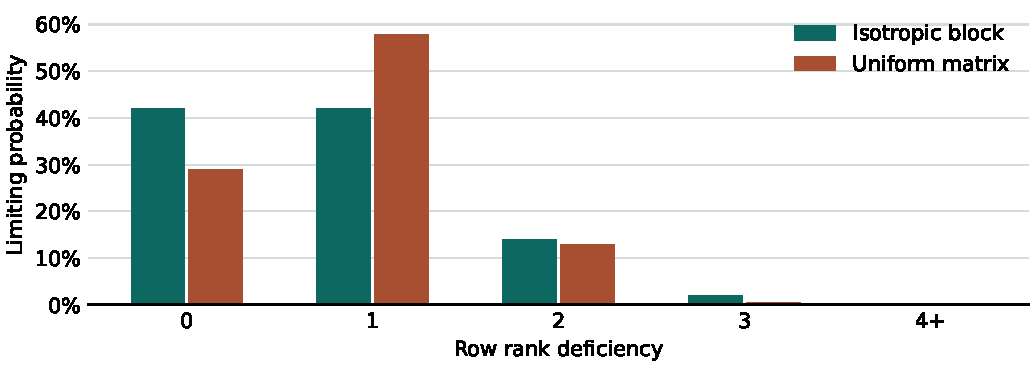
\includegraphics[width=.83\linewidth]{figures/rank_laws.pdf}
\caption{A square block over $\mathbb F_2$ with isotropic test spaces, as the ambient dimension tends to infinity. The probability of losing exactly one row of rank falls from $0.577576$ to $0.419422$. Its difference, $0.158154$, is the limiting total variation distance for the entire matrix.}
\end{figure}

The Lagrangian intersection count used when $c=0$ also appears in Richard Kueng and David Gross, \emph{Qubit stabilizer states are complex projective 3-designs}, Corollary~2 (\href{https://arxiv.org/abs/1510.02767}{arXiv:1510.02767}). The distribution comparison here concerns the full rectangular block and its distance from independent uniform entries. Ofir Gorodetsky's Theorem~1.8 in \emph{Statistics of entries of matrices from the general linear group over a finite field} treats random $\operatorname{GL}_n$ blocks (\href{https://arxiv.org/abs/2610.29305}{arXiv:2610.29305}). In that setting $n-\min(a,b)\to\infty$ suffices. Along the symplectic family just constructed this quantity grows without bound, yet the full-row-rank test detects a nonvanishing discrepancy. The symplectic result thus answers a counterpart of the finite-field block question. Its proof uses neither RH nor GRH. The boundary calculation quantifies the discrepancy at each fixed deficit in a uniform theorem. It leaves scope for finer estimates when the two specific subspaces are known.

\section{How much nonabelian information survives a support budget?}

Let $L/\mathbb Q$ be a finite Galois extension with group $G$ of order $g$, and let $N\trianglelefteq G$ have order $n$. We regard the quotient $G/N$ as already understood. For $N=[G,G]$ the fixed field $L^N$ is abelian over $\mathbb Q$, so Dirichlet GRH gives RH for its Dedekind zeta function. To apply the one-sided method one would like an observable depending on few Frobenius types. The size of its support below counts group elements, so the corresponding density of unramified rational primes is the size divided by $g$.

The incoming packet \texttt{grh\_sparse\_singular\_moduli.zip}, in \texttt{frobenius.tex}, establishes the optimal support and margin for detecting \emph{all} new characters, as well as an identity for the zero set. The question here allows the observable to discard some characters. The answer is a finite optimization over normal subgroups and determines which intermediate fields can still occur.

Call an irreducible complex character $\chi$ new if its representation is nontrivial on $N$. Consider real, inversion-invariant class functions $f$ satisfying $f(1)=0$, $0\le f\le1$ and $c_\chi=\langle f,\chi\rangle\le0$ for every new $\chi$. The coefficients are real by inversion invariance. Define the mass of the active characters by
\[
 W(f)=\sum_{\chi\ {\rm new},\ c_\chi<0}\chi(1)^2.
\]
The summands are the dimensions of the corresponding parts of the regular representation. No analytic hypothesis is needed for this optimization.

\medskip\noindent\textbf{Support-budget theorem.}
For every $0\le B\le g$,
\[
 \max_{|\operatorname{supp} f|\le B}W(f)
 =\max_{\substack{K\trianglelefteq G,\ K\subseteq N\\ n-|K|\le B}}
      \left(\frac{g}{|K|}-\frac{g}{n}\right).
\]
For each feasible $K$, the indicator $f_K=\mathbf1_N-\mathbf1_K$ attains the value attached to $K$ using exactly $n-|K|$ elements. Every admissible $f$ factors through the quotient by its zero set in $N$.

\medskip\noindent\emph{Proof.}
For $h\in N$ all quotient characters have value $\chi(1)$. By subtracting the expansion of $f(1)$ from that of $f(h)$ we get
\[
 f(h)=\sum_{\chi\ {\rm new}}(-c_\chi)(\chi(1)-\operatorname{Re}\chi(h)).
\]
Each summand is nonnegative by unitarity. The bracket vanishes exactly when $h$ acts as the identity on the representation. Thus
$K=\{h\in N:f(h)=0\}$ is the intersection of $N$ with the kernels of all active characters. It is normal in $G$. Every character appearing in $f$ kills $K$, since this holds both for the active characters and for those inflated from $G/N$. Consequently $f$ factors through $G/K$. Its support on $N$ has size $n-|K|$, and all its active characters are characters of $G/K$ outside $G/N$. The sum of their squared degrees is at most $g/|K|-g/n$ by the regular representation degree formula. Conversely, averaging a representation over a normal subgroup projects to its invariant subspace, which is either the entire representation or zero. It follows that the new-character coefficients of $f_K$ are $-|K|\chi(1)/g$ if $K$ acts trivially and zero otherwise. This proves attainment and the theorem.\hfill$\square$

\paragraph{Two exact obstructions.} For $G=S_4$, $N=A_4$, the normal subgroups of $G$ contained in $N$ are $A_4$, the Klein four-group $V_4$ and $1$. This list also follows by inspecting the possible unions of conjugacy classes of sizes $1,3,8$ and applying Lagrange's theorem. The maximum $W(f)$ is $0$ for $B<8$, $4$ for $8\le B<11$, and $22$ for $B\ge11$. At the middle value only the two-dimensional representation inflated from $S_4/V_4\simeq S_3$ can occur. The indicator of the eight $3$-cycles attains the bound. Adding the three double transpositions attains the upper step. For any nonabelian simple $G$ and $N=G$, one active character already forces support on all $g-1$ nonidentity elements. For $A_5$ this gives an all-or-nothing threshold of $59$, even if the aim is to see a single irreducible. These obstructions use the stated sign condition on every new coefficient. Arithmetic relations between specific $L$-functions can give other criteria.

\subsection*{The cost of allowing both Fourier signs}
A sparse observable might trade strictly one-sided Fourier response for a small contribution of the opposite sign. On a nonabelian simple group the loss incurred by omitting even one additional class can be bounded sharply. For $\chi\ne1$ put
\[
 \ell_\chi(h)=1-\operatorname{Re}\chi(h)/\chi(1),\qquad
 P_\pm(f)=\sum_{\chi\ne1,\ \pm c_\chi>0}|c_\chi|\chi(1).
\]
Since each nontrivial irreducible is faithful, all losses $\ell_\chi(h)$ for $h\ne1$ are positive. Define
\[
 \kappa(G)=\min_{h\ne1}
 \frac{\min_{\chi\ne1}\ell_\chi(h)}{\max_{\chi\ne1}\ell_\chi(h)}.
\]
If a nonzero real, inversion-invariant observable $0\le f\le1$ vanishes at $1$ and at some $h\ne1$, then $P_+(f)\ge\kappa(G)P_-(f)$. Indeed $f(h)-f(1)=0$ equates the negative and positive Fourier masses weighted by their respective losses at $h$. For $\kappa(G)<1$ the bound is sharp. Choose $h,\chi,\psi$ realizing the minimum ratio, and take a positive multiple of $f(u)=\ell_\chi(u)-\kappa(G)\ell_\psi(u)$. This function is nonnegative everywhere by the definition of $\kappa(G)$, and is zero at $h$ and the identity. Its two character pairs (with complex conjugates included as needed) are disjoint because their real normalized traces differ at $h$; hence $P_+/P_-=\kappa(G)$. Scale $f$ to have maximum one.

For $A_5$ the usual character table gives the minimum-to-maximum loss ratios $3/5$, $5/8$, $(10-2\sqrt5)/15$ for elements of orders $2,3,5$, respectively. At one class of $5$-cycles the extreme normalized traces are $(1+\sqrt5)/6$ for a representation of degree three and $-1/4$ for the degree-four representation. Thus omitting even one nonidentity class costs at least $(10-2\sqrt5)/15$ in the ratio $P_+/P_-$.

\paragraph{The complete rational $A_5$ calculation.}
If $f$ must be determined by the orders of Frobenius elements, write $a,b,c$ for its nonnegative values at orders $2,3,5$. These are the three possible nonidentity cycle types in the natural degree-five action. The two conjugacy classes of order five are pooled. Their character columns are exchanged by $\sqrt5\mapsto-\sqrt5$. The \href{https://www.math.rwth-aachen.de/~Thomas.Breuer/ctbllib/ctbltoc/data/A5.html}{ATLAS character table in GAP} gives the character rows on the classes $(1,2,3,5a,5b)$, with class sizes $(1,15,20,12,12)$, as follows
\[
 \begin{array}{c|rrrrr}
 &1&2&3&5a&5b\\\hline
 \chi_1&1&1&1&1&1\\
 \chi_3&3&-1&0&\phi&1-\phi\\
 \chi_{3'}&3&-1&0&1-\phi&\phi\\
 \chi_4&4&0&1&-1&-1\\
 \chi_5&5&1&-1&0&0
\end{array}
\]
where $\phi=(1+\sqrt5)/2$. Combining the two equal degree-three coefficients, the signed contributions $60\chi(1)c_\chi$ to the masses are
\[
 v_3=-90a+72c,\qquad v_4=80b-96c,\qquad v_5=75a-100b .
\]
The first term combines both degree-three representations. Sum the positive parts of these three numbers to obtain $60P_+$ and their negative parts to obtain $60P_-$. Every nonzero admissible weight has $P_->0$ since $\sum_i v_i=-15a-20b-24c$. The full frontier for the minimum ratio under a budget of $B$ group elements is
\[
\begin{array}{c|c|c}
 B & \min P_+/P_- & (a,b,c)\ \text{attaining it}\\ \hline
 0\text{--}14 & \text{no nonzero weight} & -\\
 15\text{--}19 & 5/6 &(1,0,0)\\
 20\text{--}23 & 4/5 &(0,1,0)\\
 24\text{--}34 & 3/4 &(0,0,1)\\
 35\text{--}38 & 2/3 &(1,3/4,0)\\
 39\text{--}43 & 5/8 &(4/5,0,1)\\
 44\text{--}58 & 3/5 &(0,1,5/6)\\
 59\text{--}60 & 0 &(1,1,1)
\end{array}
\]
To verify exhaustiveness, supporting only one order fixes its ratio. Below budget $59$ at most two orders can be supported. Normalize their values to sum to one. On each interval where the signs of the three $v_i$ are fixed, their ratio of linear forms is monotone or constant. Its minimum lies at an axis or a zero of some $v_i$. The three interior candidate rays are $(4,3,0)$, $(4,0,5)$ and $(0,6,5)$, yielding the table by substitution. At budget $59$ the full indicator gives $P_+=0$. The included script recomputes the rational frontier by exact arithmetic. In particular, monitoring fewer than all three nonidentity polynomial splitting types forces a positive contribution amounting to at least three fifths of the negative mass. This statement concerns the spectrum of the arithmetic observable; converting mixed Fourier signs into a conclusion on zeros needs additional information about their multiplicities.

\paragraph{Which zero problem does the optimal observable see?}
Write $M=L^K$, $F=L^N$, $m=[M:\mathbb Q]$, $a=[F:\mathbb Q]$. Suppose RH for $\zeta_F$ and fix $K\ne N$. The prime event $f_K(\operatorname{Frob}_p)=1$ means that $p$ splits completely in $F$ and fails to split completely in $M$. Write $P$ for this set of primes, omitting primes ramified in $L$, and $\delta=1/a-1/m$. Define
\[
 R_K(x)=\sum_{p\in P,\,p\le x}\log p\,(1/p-1/x)-\delta\log x-c,
\qquad B_K(s)=\sum_{p\in P}(\log p)p^{-s}.
\]
Here $c$ is the constant term of $B_K$ at $s=1$, less $\delta$. There exists $C$ with $R_K(x)\ge -C x^{-1/2}$ for all sufficiently large $x$ if and only if $\zeta_M$ satisfies RH. The ordinary Frobenius test has no access to data distinguishing individual lifts in $G$ of an element of $G/K$.

\medskip\noindent\emph{Proof.}
The regular character of a quotient counts its identity Frobenius class. Euler factors therefore give, on $\operatorname{Re}s>1$,
\[
 B_K(s)=-\frac1a\frac{\zeta_F'}{\zeta_F}(s)
         +\frac1m\frac{\zeta_M'}{\zeta_M}(s)+H(s).
\]
Here $H$ is holomorphic on $\operatorname{Re}s>1/2$, since deleting powers $p^j$, $j\ge2$, is absolutely convergent there and only finitely many ramified Euler factors are removed. The Mellin integral $\int_1^\infty R_K(x)x^{-s}\,dx$ equals
\[
 \frac{B_K(s)}{s(s-1)}-\frac{\delta}{(s-1)^2}-\frac{c}{s-1}.
\]
The pole at one cancels. At a zero $\rho$ of $\zeta_M$ with $1/2<\operatorname{Re}\rho<1$ this expression has residue $\operatorname{ord}_\rho\zeta_M/[m\rho(\rho-1)]$. In particular every real pole has negative residue. If the proposed lower bound holds, the transform of $R_K(x)+Cx^{-1/2}$, with a bounded initial interval omitted, integrates a nonnegative function. If its convergence abscissa were greater than $1/2$, Landau's theorem would force a real singularity there. The integral is positive on the real axis to the right of the abscissa, ruling out a negative-residue pole, and the continuation is regular on $[1,\infty)$. Consequently this transform is holomorphic on $\operatorname{Re}s>1/2$. A zero of $\zeta_M$ in that half-plane would produce a pole, so the functional equation proves RH.

For the forward estimate, under RH for each of $E=F,M$, the smoothed prime ideal theorem of Greni\'e and Molteni gives
$U_E(y)=\int_1^y(\psi_E(t)-t)\,dt=O_E(y^{3/2})$.
Another integration by parts gives $\int_x^\infty (\psi_E(t)-t)t^{-2}\,dt=O_E(x^{-1/2})$. Hence the prime-power ramp for $-\zeta_E'/\zeta_E$ equals $\log x$ plus a constant and $O_E(x^{-1/2})$. Omitting ramified primes changes the constant with residual $O_L((\log x)/x)$. For the higher-power terms use $\sum_{p^j\le y,\,j\ge2}\log p\ll\sqrt y$ from the elementary Chebyshev bound, first for squares, then for the $O(\log y)$ exponents at least three. Integration against $t^{-2}$ shows that deleting them changes the constant with residual $O(x^{-1/2})$. Finally the Mellin identity identifies the constant as $c$. This proves the two-sided endpoint bound.\hfill$\square$

The analytic reasoning builds on Suzuki's one-sided prime-sum criterion and the earlier incoming packets on relative races and prime sampling. Its role here is to identify the field left visible at each step of the support theorem. Establishing any required new lower bound for primes still needs arithmetic input. See \href{https://arxiv.org/abs/2411.07436}{M. Suzuki, \emph{On variants of Chebyshev's conjecture}} and \href{https://doi.org/10.1090/mcom3039}{L. Greni\'e and G. Molteni, \emph{Explicit smoothed prime ideals theorems under GRH}}.

\subsection{A quartic for which the two tests differ}
Take $L$ to be the splitting field of $f(X)=X^4-X-1$. Its discriminant is $-283$. Its reduction modulo $2$ is irreducible: it has no linear factor, and its remainder modulo $X^2+X+1$ is $1$. Hence its Galois group contains a $4$-cycle. The cubic resolvent $Y^3+4Y-1$ has no rational root. Its three roots correspond to the partitions of the four quartic roots into pairs; this gives an action transitive on three points. Thus the group order is divisible by both $4$ and $3$. A subgroup of order $12$ in $S_4$ would be the index-two subgroup $A_4$, which has no $4$-cycle. It follows that the group is $S_4$. The known abelian field is $F=\mathbb Q(\sqrt{-283})$. The intermediate normal field $M=L^{V_4}$ is the splitting field of the resolvent.

For each $p\ne283$, factor $f$ modulo $p$. The one-sided criterion gives the following two distinct problems, with a separate centering constant for each row.
\begin{center}\small
\begin{tabular}{@{}llcl@{}}\toprule
Allowed factor degrees & First primes & Density & Zero problem seen\\\midrule
$(3,1)$ & $7,11,13,23,29,\ldots$ & $1/3$ & RH for $\zeta_M$\\
$(3,1)$ or $(2,2)$ & $7,11,13,23,29,\ldots$ & $11/24$ & RH for $\zeta_L$\\\bottomrule
\end{tabular}\end{center}
The first prime distinguishing the rows is $71$, of type $(2,2)$. Of the $167$ unramified primes up to $1000$, the first row selects $59$ and the second selects $82$. These counts follow by taking $\gcd(f,X^{p^j}-X)$ modulo $p$ for $j=1,2$. For the second row, the missing theorem is the lower estimate
\[
 \sum_{\substack{p\le x\\p\text{ in the second row}}}
       (\log p)(p^{-1}-x^{-1})
 \ \ge\ \frac {11}{24}\log x+c_L-C_L x^{-1/2}
 \quad\text{for all sufficiently large }x .
\]
Here $c_L$ is prescribed by the Laurent expansion, while $C_L$ may depend on the field. A geometric bound of this form would prove RH for this particular nonabelian field. The estimates in the pinned source are for the progression and quadratic-twist weights in its construction. A comparison of twisted lattices giving the displayed quartic weight is still missing.



\section{Verification and further questions}
The accompanying index identifies the 31 GRH-related archives in the pinned incoming directory. The direct predecessors for the first two applications are \cite{fixed,packet,fieldprior}; the full-character support theorem used in Section 5 is in \cite{frobprior}. The symplectic block theorem addresses a counterpart of the general-linear problem studied by Gorodetsky \cite{goro}. These comparisons establish what was added to the supplied reports. Publication priority for the precise formulas given here has not been established.

The scripts use integer and rational arithmetic. They enumerate the small residue trees in the fixed-Gauss theorem, exhaust the residues needed for all seven quadratic $2$-adic fields, count small isotropic frames, compute the $A_5$ support table and determine quartic factorization types. Finite enumerations check the implementations and examples; the infinite ranges follow from the proofs.

\begin{enumerate}[leftmargin=1.6em,itemsep=3pt]
\item For higher $p$-power order, which ramification invariants give formulas for the positive-tolerance price as simple as the quadratic defect formula at order four? Proposition~\ref{prop:mod} supplies a finite test against which to check them.
\item For arbitrary compressed subspaces in a symplectic space, determine the limiting discrepancy in terms of the ranks of their restricted alternating forms. The isotropic boundary law gives one endpoint of that classification.
\item For the quartic in Section 5, can a geometric comparison bound the weighted count of primes of types $(3,1)$ and $(2,2)$ from below with error $O(x^{-1/2})$? The smaller event involving $(3,1)$ alone targets its cubic resolvent field's normal closure.
\end{enumerate}
\begin{thebibliography}{99}\small\raggedright
\bibitem{repo} L. Sernau and collaborators, after L. Alp\"oge with Claude. \emph{GRH for Dirichlet $L$-functions, in Lean 4}. \src{README.md}{Repository and verification status}, \src{grh/README.md}{edition checks}, \src{grh/src/Statements.lean}{public types}, \src{grh/src/Main.lean}{five exports}, \src{grh/GUIDE.md}{guide}, \src{grh/src/New/Reduction/MainInequality.lean}{main inequality}, \src{grh/src/New/Reduction/Zeros/PrimeError.lean}{Mellin residues}. The pinned project uses Lean 4.35.0 and Mathlib revision \texttt{56a00585}.
\bibitem{fixed} ProveIt, \prior{grh_exact_torsion_transfer_2026-11-25.zip}{\emph{Exact torsion specialization}}, especially \path{exact_torsion.tex} and the numerical example in \path{applications.tex}.
\bibitem{packet} ProveIt, \prior{grh-torsion-and-zero-data.zip}{\emph{How far must a torsion selector search?}}, especially \path{minimax.tex} and the questions about coefficient fields in \path{report.tex}.
\bibitem{fieldprior} ProveIt, \prior{grh-torsion-and-prime-sampling.zip}{\emph{Torsion specialization and sparse prime sums}}, especially \path{field.tex}, \path{cyclotomic.tex} and the question on noncyclotomic fields.
\bibitem{frobprior} ProveIt, \prior{grh_sparse_singular_moduli.zip}{\emph{Five-term equations for singular moduli}}, section \emph{How sparse can a one-sided Frobenius test be?}
\bibitem{kriz} D. Kriz and A. C. Nordentoft, \emph{Horizontal $p$-adic $L$-functions}, \href{https://arxiv.org/html/2310.20678v3}{Propositions 2.7 and 2.11}.
\bibitem{goro} O. Gorodetsky, \href{https://arxiv.org/abs/2610.29305}{\emph{Statistics of entries of matrices from the general linear group over a finite field}}. Related comparison for unrestricted rectangular matrices: J. Fulman and L. Goldstein, \href{https://doi.org/10.1214/13-AOP889}{\emph{Stein's method and the rank distribution of random matrices over finite fields}}.
\bibitem{analytic} M. Suzuki, \href{https://arxiv.org/abs/2411.07436}{\emph{On variants of Chebyshev's conjecture}}. L. Greni\'e and G. Molteni, \href{https://doi.org/10.1090/mcom3039}{\emph{Explicit smoothed prime ideals theorems under GRH}}, Theorem 1.1.
\end{thebibliography}
\end{document}
